\documentclass[12pt]{article}
\usepackage[utf8]{inputenc}
\usepackage[paperwidth=8.5in, paperheight=60in, margin=1.5in]{geometry}

\usepackage{graphicx}
\usepackage{pdfpages}
\usepackage{amsmath}
\usepackage{siunitx}
\numberwithin{equation}{section}
\usepackage{float}
\usepackage{subcaption}
\pagenumbering{gobble} % removes page number from TOC and pages

\usepackage{xcolor}
\definecolor{xlinkcolor}{cmyk}{1,1,0,0}
\usepackage[colorlinks,allcolors=xlinkcolor]{hyperref}
\usepackage[titles]{tocloft} % remove dots in TOC
\renewcommand{\cftdot}{}
\setcounter{tocdepth}{2}

\title{Econometrics}
\author{Andrew Lu}
\date{Mr. Lizardo, Fall 2020}

\begin{document}

    \maketitle
    \label{sec:top}
    \tableofcontents

\section{Introduction to Statistics}

\subsection{Mean}
\begin{align}
    \mu=\frac{\sum\limits_{i=1}^{N}{x_i}}{N} \\
    \overline{X}=\frac{\sum\limits_{i=1}^{N}{x_i}}{n}
\end{align}

\subsection{Variance}
\begin{align}
    \sigma^2=\frac{\sum\limits_{i=1}^{N}{(x_1-\mu)^2}}{N} \\
    s^2=\frac{\sum\limits_{i=1}^{n}{(x_1-\Bar{x})^2}}{n-1}
\end{align}
where $\sigma^2=$ population variance and $s^2=$ sample variance. The denominator is $n-1$ for sample variance calculations because of degrees of freedom.

\subsection{Standard Deviation}
\begin{align}
    \sigma=\sqrt{\frac{\sum\limits_{i=1}^{N}{(x_1-\mu)^2}}{N}} \\
    s=\sqrt{\frac{\sum\limits_{i=1}^{n}{(x_1-\Bar{x})^2}}{n-1}}
\end{align}

\subsection{Data Distribution}
\subsubsection{Histograms}
\begin{figure}[!ht]
    \centering
    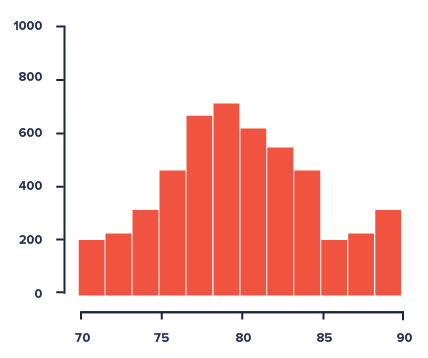
\includegraphics[width=0.6\linewidth]{figures/histogram.png}
\end{figure}

\subsubsection{Box Plots}
\begin{figure}[!ht]
    \centering
    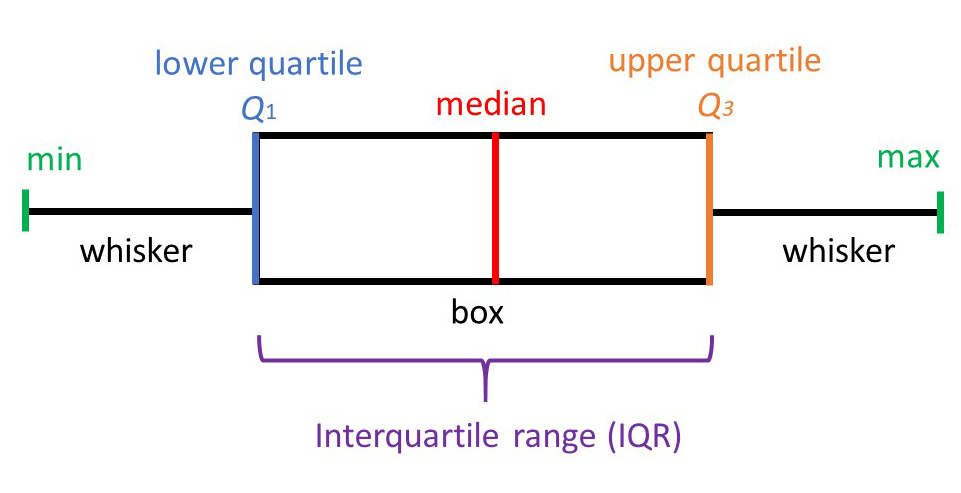
\includegraphics[width=0.8\linewidth]{figures/boxplot.jpg}
\end{figure}
Outliers: any value outside 1.5 $\times$ IQR above Q3 or below Q1
\begin{align}
    IQR = Q3 - Q1
\end{align}

\subsubsection{SOCS}
\begin{enumerate}
    \item Symmetry: positive/right skew, negative/left skew, or normal curve
    \item Outliers: skew the distribution in its direction
    \item Center: mean = balancing point, median = data split in half
    \item Spread: outliers affect spread by impacting skew
\end{enumerate}
\begin{figure}[!ht]
    \centering
    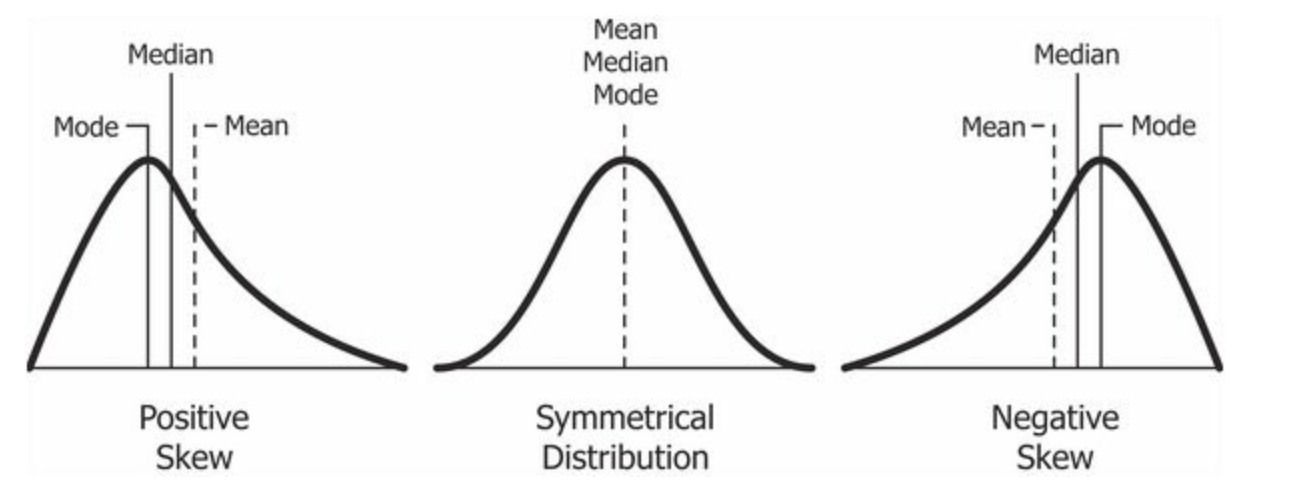
\includegraphics[width=0.9\linewidth]{figures/skew.png}
\end{figure}

\subsection{Probability}
\begin{enumerate}
    \item Conditional Probability:
    \begin{align}
        P(A|B) = \frac{P(A \cap B)}{P(B)}
    \end{align}
\end{enumerate}

\section{Random Variables}

\subsection{Discrete Random Variables}
\subsubsection{Measures}
\begin{gather}
    \mu_x = \sum x \times p(x) \\
    \sigma^2_x = (x_1-\mu_x)^2 p_1 + (x_2-\mu_x)^2 p_2 + ... + (x_i-\mu_x)^2 p_i
\end{gather}

\subsubsection{Binomial Situations}
\begin{enumerate}
    \item B: Binary Outcomes
    \item I: Independent Trials
    \item N: Number of Trials
    \item S: Success Probability
\end{enumerate}
\subsubsection{Binomial Probabilities}
\begin{gather}
    P(k)=\binom{n}{k} p^k (1-p)^{n-k} \\
    \sigma = \sqrt{np(1-p)}
\end{gather}

\subsection{Continuous Random Variables}
%\subsubsection{Probability Density Function}
%\subsubsection{Area Under Curve (AUC)}
\subsubsection{Normal Distribution}
\begin{figure}[!ht]
    \centering
    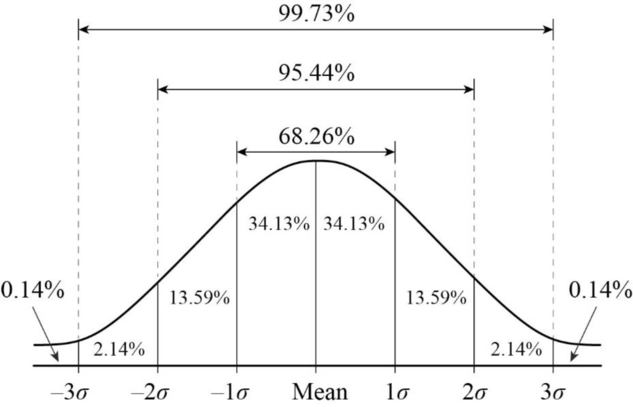
\includegraphics[width=0.8\linewidth]{figures/normalcurve.png}
\end{figure}

\subsubsection{Z-Score}
\begin{gather}
    \text{z-score: } z = \frac{x-\mu}{\sigma}
\end{gather}

\begin{figure}[!ht]
    \centering
    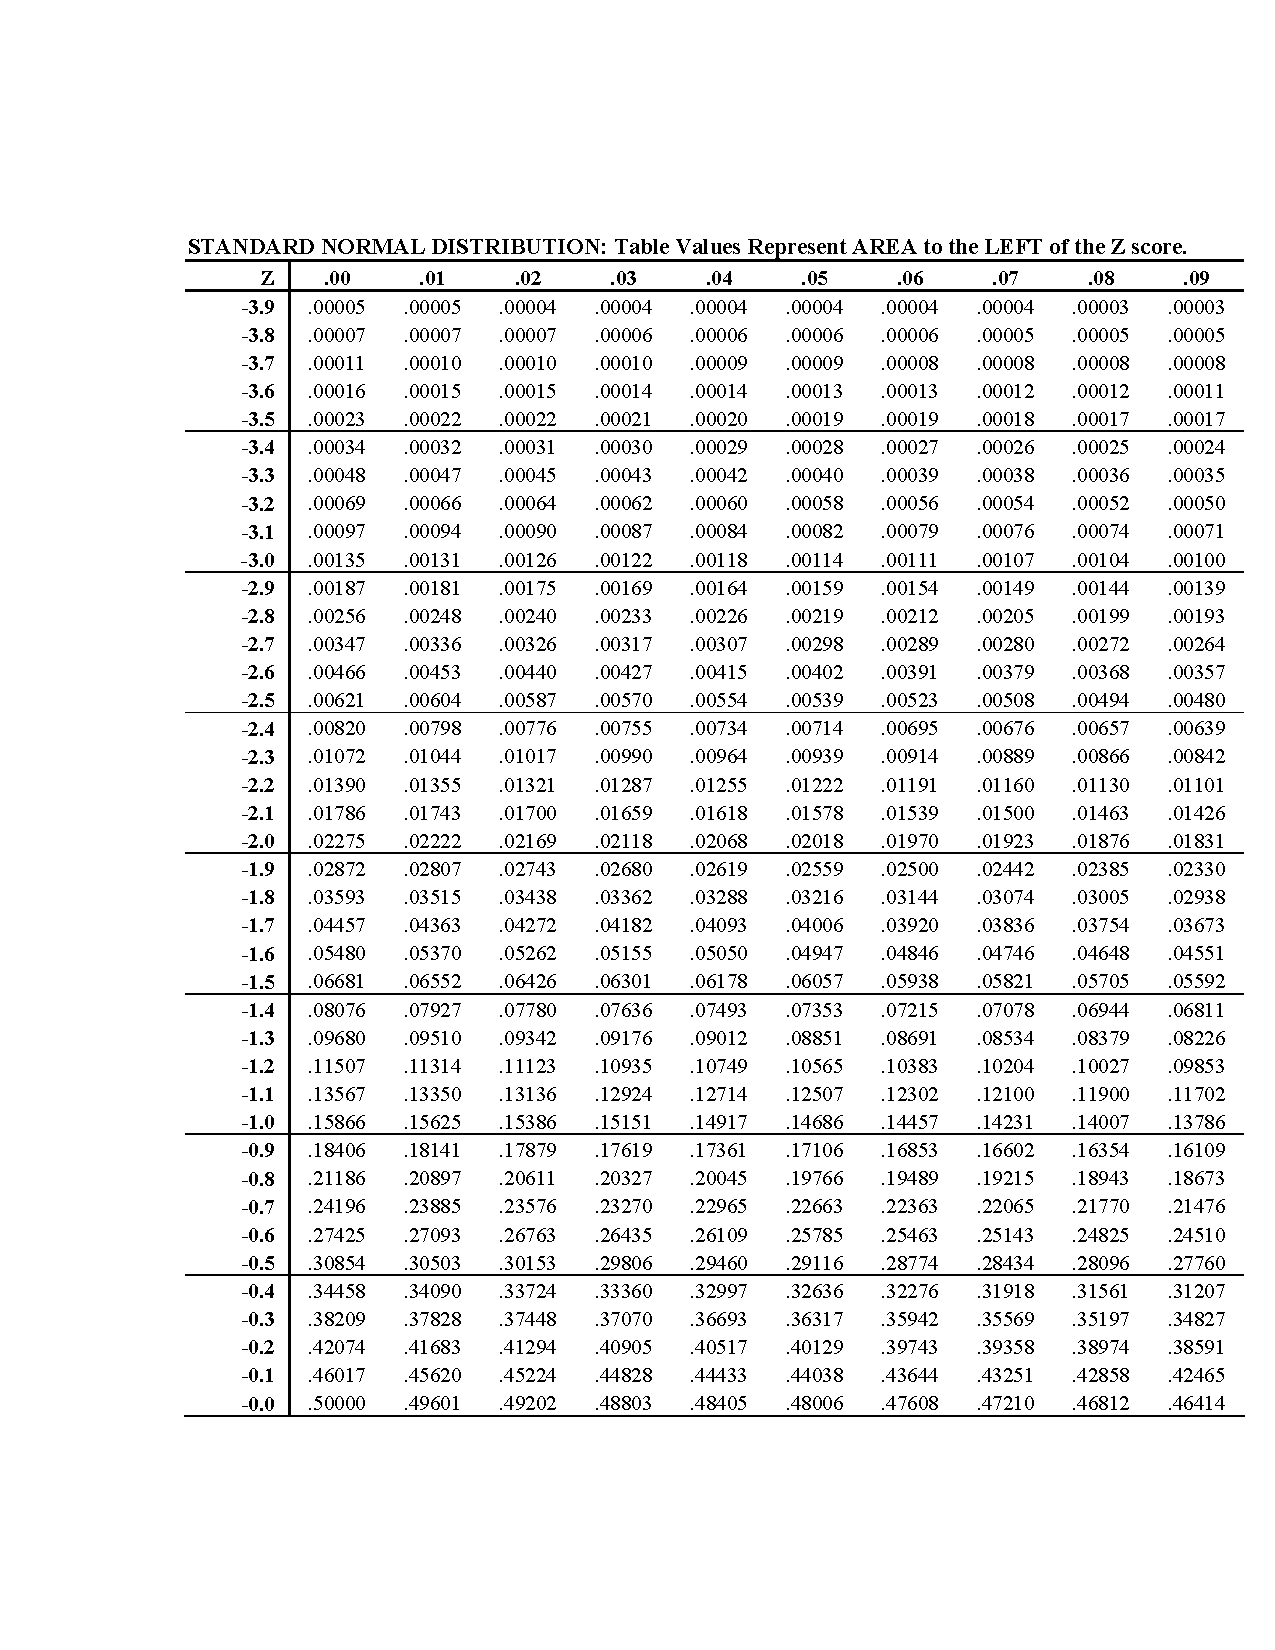
\includegraphics[page=1, width=0.9\linewidth, trim=4cm 4cm 1.25cm 4cm]{standardnormaltable.pdf}
    \label{zscore}
\end{figure}

\begin{figure}[!ht]
    \centering
    \includegraphics[page=2, width=0.9\linewidth, trim=4.1cm 4cm 1.15cm 4cm]{standardnormaltable.pdf}
\end{figure}

% 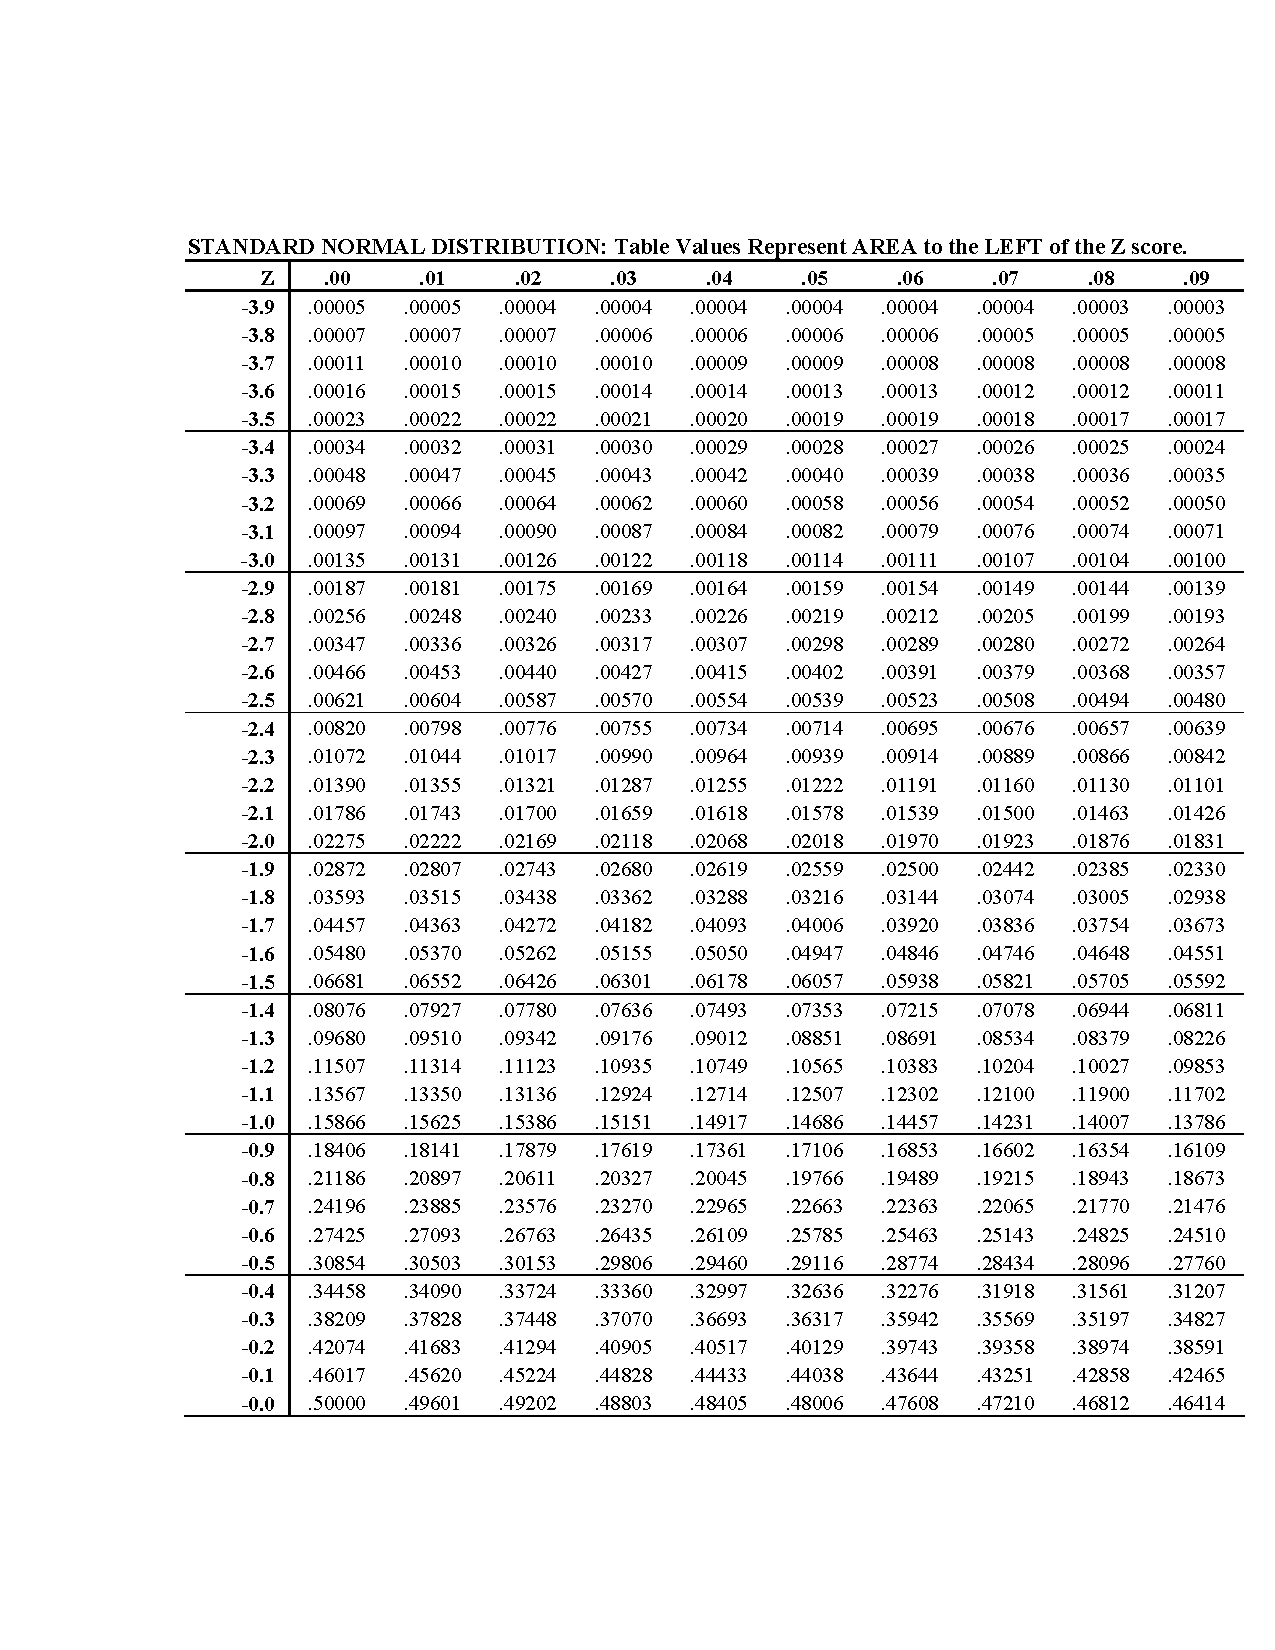
\includepdf[]{standardnormaltable.pdf}

\noindent \begin{flushright} \hyperref[sec:top]{back to top} \end{flushright}
\end{document}
